Fig.~\ref{fig:markov_first} shows  first-order Markov models of the flies' turning behavior. These models show whether there is a ``memory'' of the last turning direction.

The model has two states: `last left', and `last right', depending of what was the direction of the last saccade. The states are indicated by circles. Inside each circle, there is a percentage indicating the fraction of time spent in each state. 
Most of the percentage are around 50\%, meaning that the flies do not have an average preference for turning left or right.

Each state has two transitions, corresponding to the next action (turning right or left). The corresponding transition probability is shown as well.

From these plots, we notice two clear phenomena:

\begin{itemize} 
	\item  Successive saccades are very correlated. If the flies turns left, it is likely that it will keep turning left.
	
	\item  The statistics are all very symmetric: left or right does not make a difference.
	
\end{itemize}

Preliminary results of the free-flight data showed an inverse correlation: if the last turn was towards left, the next was much more likely to be to the right.  This is shown in  Fig.~\vref{fig:ff-markov_first}. 

\subsection*{Caveats}
\begin{itemize}
	\item I did this analysis before noticing the results in Fig.~\ref{fig:sac_sign_averages}. I was assuming that the data was much more homogenous. Therefore, probably this analysis must be corrected in some way. For example, by only including the logs in which the flies act ``normal'' enough.
\item The data in Fig.~\ref{fig:ff-markov_first} were obtained with another saccade detector, and I did not do all the manual labeling and ROC analysis. Therefore it is not as reliable as the tethered data.
\end{itemize}
\vfill
\begin{figure}[h!]
	\centering
	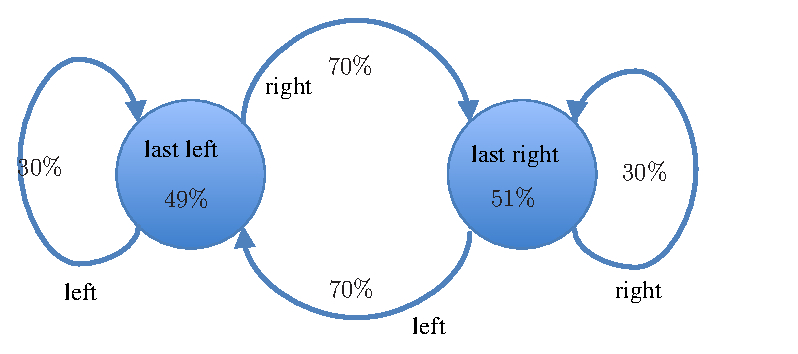
\includegraphics[width=6cm]{../comments/freeflight/markov_first}
	\caption{ \label{fig:ff-markov_first}  \Dmelanogaster (Mamarama) }
\end{figure}
